\documentclass[10pt]{article}
\usepackage[paperwidth=12cm,paperheight=6.5cm,margin=5mm]{geometry}
\usepackage{tikz}
\pagestyle{empty}

\begin{document}
\centering
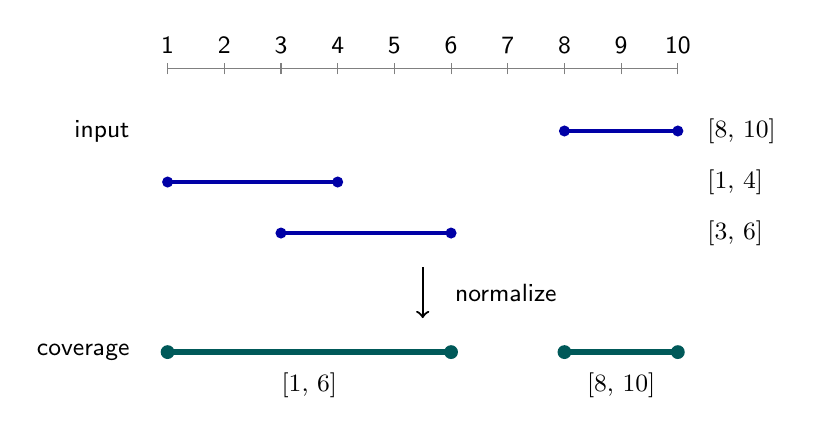
\begin{tikzpicture}[x=0.72cm,y=0.72cm,font=\sffamily\small]
  \draw[gray] (1,4.1) -- (10,4.1);
  \foreach \point in {1,...,10} {
    \draw[gray] (\point,4.0) -- (\point,4.2);
    \node[above] at (\point,4.2) {\point};
  }

  \node[anchor=east] at (0.5,3) {input};
  \foreach \lowerpoint/\upperpoint/\row in {8/10/3,1/4/2.1,3/6/1.2} {
    \draw[blue!65!black,line width=1.2pt] (\lowerpoint,\row) -- (\upperpoint,\row);
    \fill[blue!65!black] (\lowerpoint,\row) circle[radius=2pt];
    \fill[blue!65!black] (\upperpoint,\row) circle[radius=2pt];
    \node[anchor=west] at (10.35,\row) {$[\lowerpoint,\,\upperpoint]$};
  }

  \draw[->,line width=0.8pt] (5.5,0.6) -- (5.5,-0.3);
  \node[anchor=west] at (5.9,0.15) {normalize};

  \node[anchor=east] at (0.5,-0.9) {coverage};
  \foreach \lowerpoint/\upperpoint in {1/6,8/10} {
    \draw[teal!70!black,line width=2pt] (\lowerpoint,-0.9) -- (\upperpoint,-0.9);
    \fill[teal!70!black] (\lowerpoint,-0.9) circle[radius=2.5pt];
    \fill[teal!70!black] (\upperpoint,-0.9) circle[radius=2.5pt];
    \node[below] at ({(\lowerpoint+\upperpoint)/2},-1.1)
      {$[\lowerpoint,\,\upperpoint]$};
  }
\end{tikzpicture}
\end{document}
